\documentclass[a4paper, 14pt]{article}
\usepackage[margin=1.6cm]{geometry}
\usepackage[utf8]{inputenc}
\usepackage{minted}
\usepackage[russian]{babel}
\usepackage{amsmath}
\usepackage{graphicx}
\usepackage{changepage}
\usepackage{hyperref}
\usepackage{cases}
\usepackage{tikz-timing}[2017/12/20]
\usepackage{relsize}
\usepackage{booktabs}
\usepackage{gensymb}
\usepackage{multirow}
\usepackage{longtable}
\usetikzlibrary {arrows.meta}

\hypersetup{
	linkbordercolor = {1 1 1}
}

\usepackage{tikz-timing}[2009/05/15]
\usepackage{multicol}
\usepackage[T2A]{fontenc}
\usepackage{pgfplots}
%\usepackage[left=2.5cm, right=1.5cm, vmargin=2.5cm]{geometry}
\setlength\parindent{0pt} % Удалить отступы из параграфов.

\usepackage{listings}
\usepackage{caption}
\DeclareCaptionFont{white}{\color{white}} % Текст заголовка.
\DeclareCaptionFormat{listing}{\colorbox{gray}{\parbox{\textwidth}{#1#2#3}}}
\captionsetup[lstlisting]{format=listing,labelfont=white,textfont=white}
\renewcommand\labelenumi{\theenumi)}
\setlength\parindent{24pt}



\begin{document}
\lstset{
    language=java,                 % Выбор языка для подсветки (здесь это java).
    basicstyle=\small\sffamily,    % Размер и начертание шрифта для подсветки кода.
    numbers=left,                  % Где поставить нумерацию строк (слева\справа).
    numberstyle=\tiny,             % Размер шрифта для номеров строк.
    stepnumber=1,                  % Размер шага между двумя номерами строк.
    firstnumber=1,
    numberfirstline=true
    numbersep=5pt,                 % Как далеко отстоят номера строк от подсвечиваемого кода.
    backgroundcolor=\color{white}, % Цвет фона подсветки - используем \usepackage{color}.
    showspaces=false,              % Показывать или нет пробелы специальными отступами.
    showstringspaces=false,        % Показывать или нет пробелы в строках.
    showtabs=false,                % Показывать или нет табуляцию в строках.
    frame=single,                  % Рисовать рамку вокруг кода.
    tabsize=2,                     % Размер табуляции по умолчанию равен 2 пробелам.
    captionpos=t,                  % Позиция заголовка вверху [t] или внизу [b].
    breaklines=true,               % Автоматически переносить строки (да\нет).
    breakatwhitespace=false,       % Переносить строки только если есть пробел.
    escapeinside={\%*}{*)}         % Если нужно добавить комментарии в коде.
}

\begin{titlepage}
    \center

    ФЕДЕРАЛЬНОЕ ГОСУДАРСТВЕННОЕ АВТОНОМНОЕ ОБРАЗОВАТЕЛЬНОЕ УЧРЕЖДЕНИЕ ВЫСШЕГО ОБРАЗОВАНИЯ\linebreak
    «Санкт-Петербургский политехнический университет Петра Великого»
    \noindent\rule{500pt}{0.8pt} \\
    \textsc{\Large Институт компьютерных наук и кибербезопасности}\\
    \textsc{\large Высшая школа программной инженерии}\\[1.5cm]

    { \huge \bfseries ОТЧЕТ ПО СИСТЕМНОМУ ТЕСТИРОВАНИЮ	\\
    \Large \mdseries АГРЕГАТОР ЦИФРОВЫХ ФИНАНСОВЫХ АКТИВОВ <<ТЕССЕРАКТ>> \\
    \large по дисциплине <<Технологии разработки качественного программного обеспечения>>}\\
    \flushright{
        {\phantom{qwe}}\\[1.0cm]
    }

    \begin{figure}[H]
        \centering
        
\includegraphics[width=10cm]{./resources/1.png}\\[2.0cm]
    \end{figure}

    \begin{multicols}{2}
        \begin{flushright} \large

            {Выполнили студенты группы: 5130904/00104:}\\
            {\phantom{qwe}}\\
            {\phantom{qwe}}\\
            {\phantom{qwe}}\\
            {\phantom{qwe}}\\

            {Преподаватель:\\}

        \end{flushright}
        \begin{flushright}

            {Почернин В. С.}\\
            {Шиляев В. С.}\\
            {Мурзаканов И. М.}\\
            {Разукрантов В. Е.}\\[0.5cm]


            Маслаков А. П.\\

        \end{flushright}
    \end{multicols}

    \flushright{
        {\phantom{qwe}}\\[0.5cm]
    }
    \centering{
        Санкт-Петербург\\
        2024
    }

    \vfill
\end{titlepage}

\Large
\tableofcontents
\newpage
\large

\section{Постановка задачи}

На данном уровне необходимо протестировать готовый продукт по 
бизнес-требованиям, сформированным перед началом непосредственного 
проектирования программного продукта. В качестве тестовых сценариев 
выбираются основные сценарии использования ПО в полностью рабочем 
окружении. Целесообразно использование инструментов веб-тестирования 
или UI-тестирования, таких как selenium, puppeteer и т. д.

Минимальное количество сценариев - 10.

\subsection{Обязательные требования}

\begin{enumerate}
    \item Предварительное формирование документа, описывающего тестовые сценарии.
    \item Поднятие сервера непрерывной интеграции и запуск задачи системного тестирования по временному триггеру или в ручном режиме.
\end{enumerate}

\subsection{Содержание отчета}

Отчет по интеграционному тестированию должен содержать:

\begin{enumerate}
    \item Отчет о выполненной работе, использованных инструментах.
    \item Тест-план со словесным описанием тестовых сценариев.
    \item Отчет о прохождении тестов с результатами на сервере непрерывной интеграции.
\end{enumerate}

\section{Ход работы}

\subsection{Отчет о выполненной работе, использованных инструментах}

В рамках проведенной работы, код клиентской части приложения был покрыт системными тестами.

\subsubsection{Использованные инструменты}

Были использованы следующие инструменты:

\begin{itemize}
    \item \texttt{JUnit} - фреймворк для языков программирования \texttt{Java} и \texttt{Kotlin}, предназначенный для автоматического unit-тестирования. Данный фреймворк позволяет удобно создавать, организовывать и выполнять тесты, благодаря широкому набору аннотаций и встроенной поддержки в популярных IDE. Для клиентской части применялся \texttt{JUnit4}.
    \item \texttt{Compose UI Test} - - это библиотека, предоставляемая Android Jetpack для тестирования пользовательского интерфейса (UI) в приложениях, использующих Jetpack Compose. Эта библиотека предоставляет набор инструментов и API для написания и выполнения автоматизированных тестов, которые проверяют корректность работы пользовательского интерфейса приложений, созданных с использованием Jetpack Compose.
    \item \texttt{GitHub Actions} - система непрерывной интеграции (\texttt{CI}), используемая нами для автоматического выполнения тестов при открытии \texttt{PR} или мерже в мастер ветку. Позволяет автоматизировать процесс интеграционного тестирования и не только.
\end{itemize}

\subsection{Тест-план со словесным описанием тестовых сценариев}

Описание тест-плана удобно разделить на несколько категорий.

\textbf{Для залогиненного пользователя}
\subsubsection{AssetTest}

В данном разделе описаны тесты, связанные с Активами.

\begin{enumerate}
    \item \texttt{whenGoToAsset\_thenAssetIsLoadedSuccessfully} - получение информации по выбранному активу.
    
    \texttt{Порядок действий:}
    
    1. Нажать на любой актив.
    
    2. Проверить, что описание отображается корректно.
    \item \texttt{whenSwipeUp\_thenAllAssetsAreShown} - прогрузка активов и проверка отображаемого количества.

    \texttt{Порядок действий:}
    
    1. Выполнять свайп вверх, пока не будет достигнут конец списка.
    
    2. Проверить, что количество активов соответствует количеству активов в тестовой базе.
    
\end{enumerate}

\subsubsection{FavoriteTest}

В данном разделе описаны тесты, связанные с Избранным.

\begin{enumerate}
    \item \texttt{whenAddFavorite\_thenAssetIsAddedToFavorites} - добавление актива в избранные.

    \texttt{Порядок действий:}
    
    1. Нажать на кнопку «В избранное» около актива.
    
    2. Перейти на вкладку «Избранное».

    3. Проверить, что количество активов равно 1.
    
\end{enumerate}

\subsubsection{DiversificationTest}

В данном разделе описаны тесты, связанные с Диверсификациями.

\begin{enumerate}
    \item \texttt{whenGoToDiversification\_thenDiversificationAssetsAreShown} - получить активы своей диверсификации.

    \texttt{Порядок действий:}
    
    1. Перейти на вкладку «Диверсификации».
    
    2. Нажать на диверсификацию.

    3. Проверить, что активы показываются.
    \item \texttt{givenValidAmount\_whenCreateDiversification\_thenDiversificationIsCreated} - создать диверсификацию с корректными данными.

    \texttt{Порядок действий:}
    
    1. Перейти на вкладку «Диверсификации».
    
    2. Нажать на кнопку «Создать диверсификацию».

    3. Ввести сумму «10000».

    4. Нажать на кнопку «Создать диверсификацию».

    5. Проверить, что количество диверсификаций равно 2.
    \item \texttt{givenAmountSmallerThanMinPrice\_whenCreateDiversification\_thenErrorDialogIsShown} - создание диверсификации с указанием некорректной суммы диверсификации.

    \texttt{Порядок действий:}
    
    1. Перейти на вкладку «Диверсификации».
    
    2. Нажать на кнопку «Создать диверсификацию».

    3. Ввести сумму «1».

    4. Нажать на кнопку «Создать диверсификацию».

    5. Проверить, что показывается сообщение об ошибке.
    
\end{enumerate}

\subsubsection{ChangePasswordTest}

В данном разделе описаны тесты, связанные с Изменением пароля.

\begin{enumerate}
    \item \texttt{givenValidDetails\_whenChangePassword\_thenPasswordIsChanged} - изменение пароля с указанием корректных данных.

    \texttt{Порядок действий:}
    
    1. Перейти на вкладку «Настройки».
    
    2. Ввести корректный старый пароль.

    3. Ввести корректный новый пароль.

    4. Ввести корректное подтверждение пароля.

    5. Нажать на кнопку «Изменить пароль».

    6. Проверить, что показывается сообщение об успехе.

    7. Закрыть сообщение.

    8. Нажать на кнопку «Выйти из аккаунта».

    9. Ввести корректный логин.

    10. Ввести старый пароль.

    11. Нажать на кнопку «Войти».

    12. Проверить, что показывается сообщение об ошибке.

    13. Закрыть сообщение.

    14. Ввести новый пароль.

    15. Нажать на кнопку «Войти».

    16. Проверить, что вход выполнен успешно.
    
    \item \texttt{givenInvalidOldPassword\_whenChangePassword\_thenErrorDialogIsShown} - изменение пароля с указанием некорректных данных.

    \texttt{Порядок действий:}
    
    1. Перейти на вкладку «Настройки».
    
    2. Ввести некорректный старый пароль.

    3. Ввести корректный новый пароль.

    4. Ввести корректное подтверждение пароля.

    5. Нажать на кнопку «Изменить пароль».

    6. Проверить, что показывается сообщение об ошибке.
\end{enumerate}

\textbf{Для незалогиненного пользователя}
\subsubsection{LoginTest}

В данном разделе описаны тесты, связанные с входом в приложение.

\begin{enumerate}
    \item \texttt{givenValidDetails\_whenLogin\_thenLoginIsSuccessful} - вход в приложение с использованием корректного логина и пароля.

    \texttt{Порядок действий:}
    
    1. Ввести корректный логин.
    
    2. Ввести корректный пароль.

    3. Проверить, что вход выполнен успешно.
    \item \texttt{givenInvalidPassword\_whenLogin\_thenLoginIsUnsuccessful} - вход в приложение с использованием некорректного пароля.

    \texttt{Порядок действий:}
    
    1. Ввести корректный логин.
    
    2. Ввести некорректный пароль.

    3. Проверить, что показывается сообщение об ошибке.
\end{enumerate}

\subsubsection{RegisterTest}

В данном разделе описаны тесты, связанные с регистрацией.

\begin{enumerate}
    \item \texttt{givenValidDetails\_whenRegister\_thenRegistrationIsSuccessful} - регистрация в приложении с использованием корректных данных.

    \texttt{Порядок действий:}
    
    1. Перейти на страницу регистрации.
    
    2. Ввести корректный логин.

    3. Ввести корректный email.

    4. Ввести корректный пароль.

    5. Ввести корректное подтверждение пароля.

    6. Нажать на кнопку «Зарегистрироваться».

    7. Проверить, что показывается сообщение об успехе.

    8. Ввести корректный логин.

    9. Ввести корректный пароль.

    10. Проверить, что вход выполнен успешно.
    \item \texttt{givenDuplicateLogin\_whenRegister\_thenErrorDialogIsShown} - регистрация в приложении с использованием логина-дубликата.
    
    \texttt{Порядок действий:}
    
    1. Перейти на страницу регистрации.
    
    2. Ввести логин-дубликат.

    3. Ввести корректный email.

    4. Ввести корректный пароль.

    5. Ввести корректное подтверждение пароля.

    6. Нажать на кнопку «Зарегистрироваться».

    7. Проверить, что показывается сообщение об ошибке.
\end{enumerate}

\subsection{Отчет о прохождении тестов с результатами на сервере непрерывной интеграции}

За работу сервера непрерывной интеграции отвечает конфигурационный файл \texttt{e2e\_tests.yml}:
\small
\inputminted[frame=single]{yaml}{./code/e2e_tests.yml}
\large

Как можно заметить, мы выполняем следующие шаги:

\begin{itemize}
    \item Копируем наш репозиторий в систему непрерывной интеграции.
    \item Включаем поддержку KVM для ускорения запуска виртуальных машин.
    \item Устанавливаем виртуальную машину \texttt{Java}.
    \item Устанавливаем \texttt{Gradle}.
    \item Восстанавливаем кэш Android Virtual Device для ускорения создания эмуляторов Android.
    \item Создаем Android Virtual Device.
    \item Собираем backend с помощью \texttt{Gradle}.
    \item Заменяем реальные файлы миграций тестовыми.
    \item Запускаем  \texttt{PostgreSQL} базу данных с помощью \texttt{Docker Compose}.
    \item Запускаем backend приложение.
    \item Запускаем end-to-end тесты для Android приложения.
    \item Загружаем артефакты тестов в систему интеграции.
\end{itemize}

Как можно заметить, запуск данного сценария происходит при следующих условиях:

\begin{itemize}
    \item Произошел пуш в мастер-ветку.
    \item Открылся \texttt{PR} в мастер-ветку.
\end{itemize}

Страница с пройденным \texttt{CI} выглядит следующим образом:

\begin{figure}[H]
    \centering
    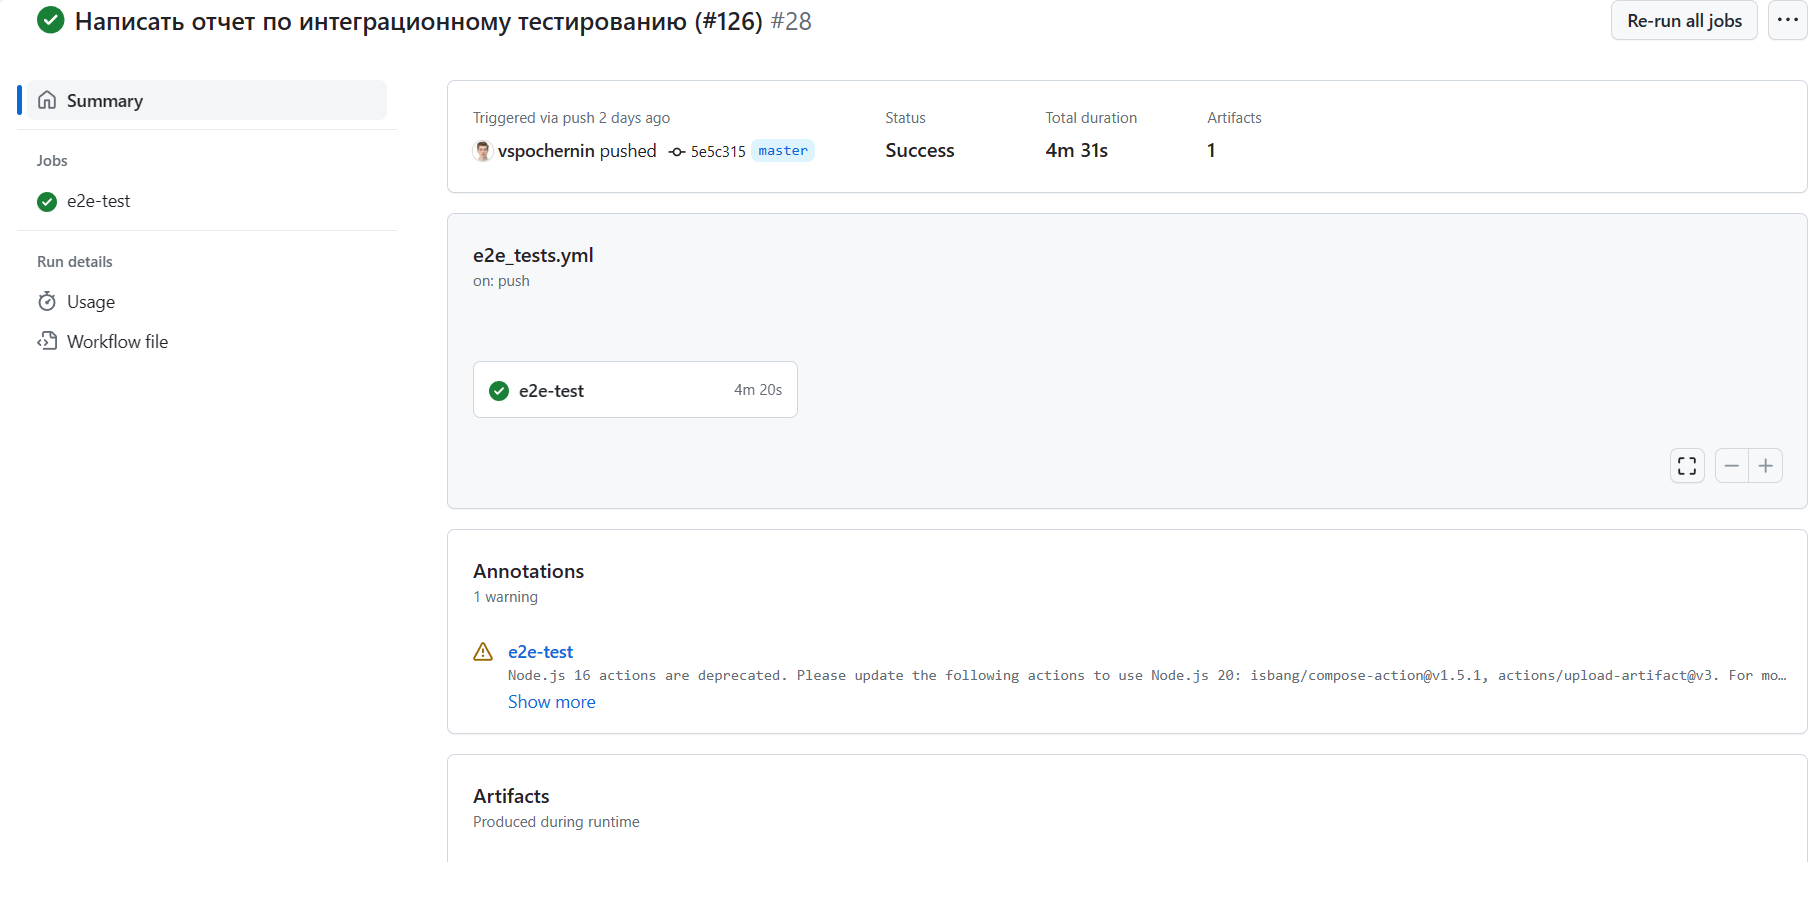
\includegraphics[width=17cm]{resources/2.png}\\
    \caption{Пройденный \texttt{CI}}
\end{figure}

Ниже можно скачать архив с артефактами тестирования. Он содержит в себе \texttt{HTML}-страницу с подробным отчетом о пройденных тестах.

\begin{figure}[H]
    \centering
    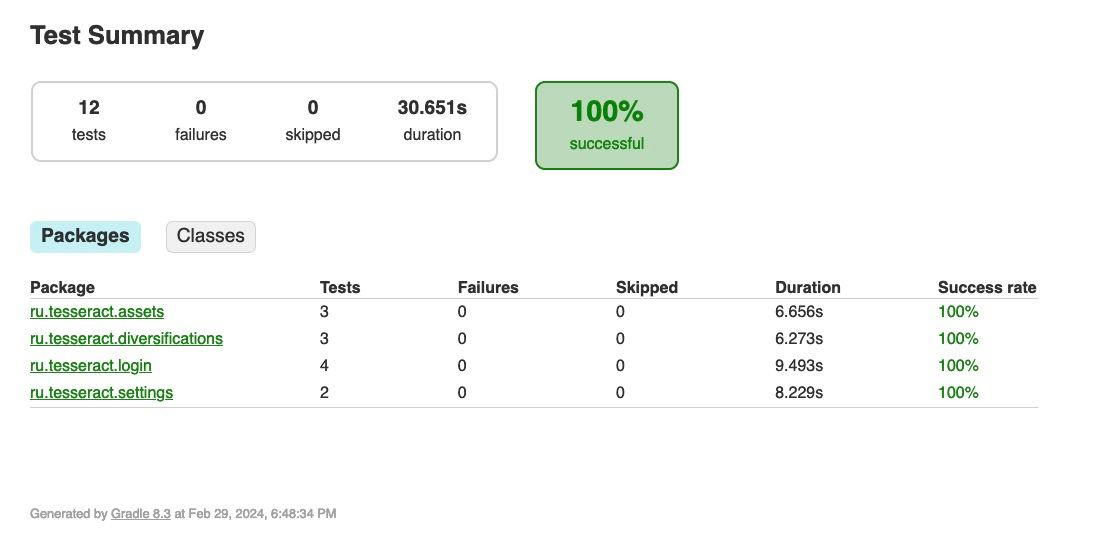
\includegraphics[width=15cm]{resources/3.jpg}\\
    \caption{Отчет о пройденных тестах}
\end{figure}

\end{document}